% compile this file with xelatex
\documentclass[12pt]{article}
\usepackage{graphicx}
\usepackage[margin=2cm, a4paper]{geometry}
\usepackage{setspace}
\usepackage{pdfpages}
\usepackage{float}
\usepackage{ctex}
\usepackage{amsmath}
\usepackage{fancyvrb}
\usepackage{amssymb}
\usepackage{minted}
\usepackage{enumitem}
\usepackage[colorlinks,linkcolor=blue]{hyperref}

\usepackage{xeCJK}
\setCJKmainfont{Noto Sans TC}

\renewcommand{\contentsname}{Contents}
\renewcommand{\figurename}{Figure}
\renewcommand{\tablename}{Table}
\hypersetup{
    colorlinks=true,
    linkcolor=black,
    filecolor=magenta,      
    urlcolor=blue,
}
\newcommand{\mytitle}{網路管理與系統管理 HW 11}
\newcommand{\myauthor}{B13902022 賴昱錡}

\usepackage{fancyhdr}
\pagestyle{fancy}
\fancyhead{}
\fancyhead[L]{\mytitle}
\fancyhead[R]{\myauthor}

\title{\mytitle}
\author{\textbf{\myauthor}}
\date{\today}

\begin{document}

% \doublespacing
\maketitle

\section*{1. 三角準則的侵略者!?}
\subsection*{(a)}
\begin{enumerate}
    \item 2017 年的勒索病毒 Wanacry 全球災情,被病毒感染時,電腦中檔案會被加密,必須支付比特幣才有可能解鎖。違反 CIA 三項,因為駭客能遠端存取、操作你的檔案 (違反 C),電腦的檔案或服務也可能毀壞、變得不完整 (違反 IA)。
    \item Crazy Hunter 組織透過 USB 的途徑感染電腦,駭得馬偕醫院的病患資料。違反 CIA 中的 Confidentiality,因為病患的病例與身份皆為相當敏感、重要,應被更多加密與保護的資訊。
\end{enumerate}
\subsection*{(b)}
\noindent \textbf{Assumption:}

\noindent 筆電的硬體設備無故障 (且記憶體、硬碟容量夠)

\noindent \textbf{Threat Model:}

\begin{center}
\begin{tabular}{ |c|c| } 
 \hline
 Threat Model & Countermeasure \\
 \hline
 有人嘗試從旁偷窺密碼 & 安裝螢幕防窺片 \\ 
 \hline
 有人使用暴力破解密碼 (大量輸入) & 採用指紋/臉部辨識解鎖 \\ 
 \hline
\end{tabular}
\end{center}
\subsection*{(c)}
\noindent \textbf{Assumption:}

\noindent 傳送簡訊時,必定可以成功發送

\noindent \textbf{Threat Model:}

\begin{center}
\begin{tabular}{ |p{0.4\linewidth}|p{0.4\linewidth}| } 
 \hline
 Threat Model & Countermeasure \\
 \hline
 簡訊內容可以被偽造 (可以在 A 地點,傳送 B 地點條碼所生的簡訊) & 使用 GPS 定位使用者的傳送地點 \\ 
 \hline
 有人手動修改簡訊內容,誤導也浪費實名制系統的資源 & 對簡訊的格式嚴格過濾(不符合格式的無法傳送) \\ 
 \hline
\end{tabular}
\end{center}
\subsection*{(d)}
\noindent \textbf{Assumption:}

\noindent 1. 所有人的電腦、網路介面均能正常運作

\noindent 2. 考生無法連上任何通訊軟體 (Gmail, Discord...etc)

\noindent \textbf{Threat Model:}

\begin{center}
\begin{tabular}{ |p{0.4\linewidth}|p{0.4\linewidth}| } 
 \hline
 Threat Model & Countermeasure \\
 \hline
 有人透過工作站的 \verb|/tmp2/| 存放作答資訊 & 令考生暫時只能修改home,封鎖其特定folder的權限 \\ 
 \hline
 有人試著偽造其他組的 token,幫他們作答 & 作答前組員會取得 OTP,表單須繳交該份 OTP 才算有效 \\ 
 \hline
\end{tabular}
\end{center}

\newpage
\section*{2. 果汁店也有洞 (20 pts)}
\subsection*{(a)}
\begin{figure}[H]
    \centering
    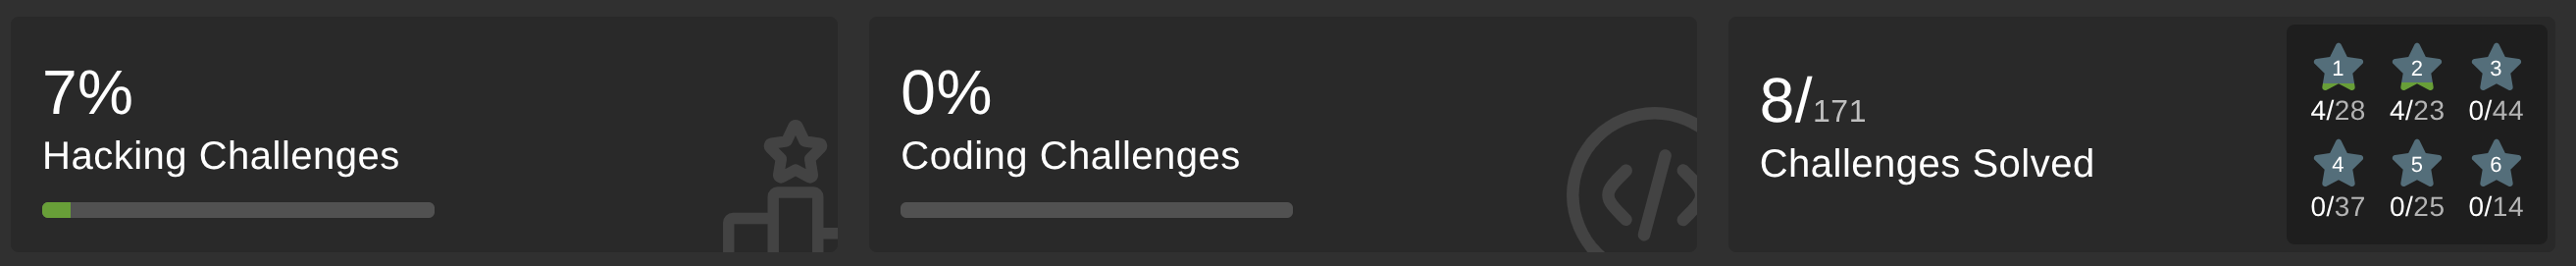
\includegraphics[width=0.5\linewidth]{image copy 3.png}
    % \caption{Caption}
\end{figure}
\begin{figure}[H]
    \centering
    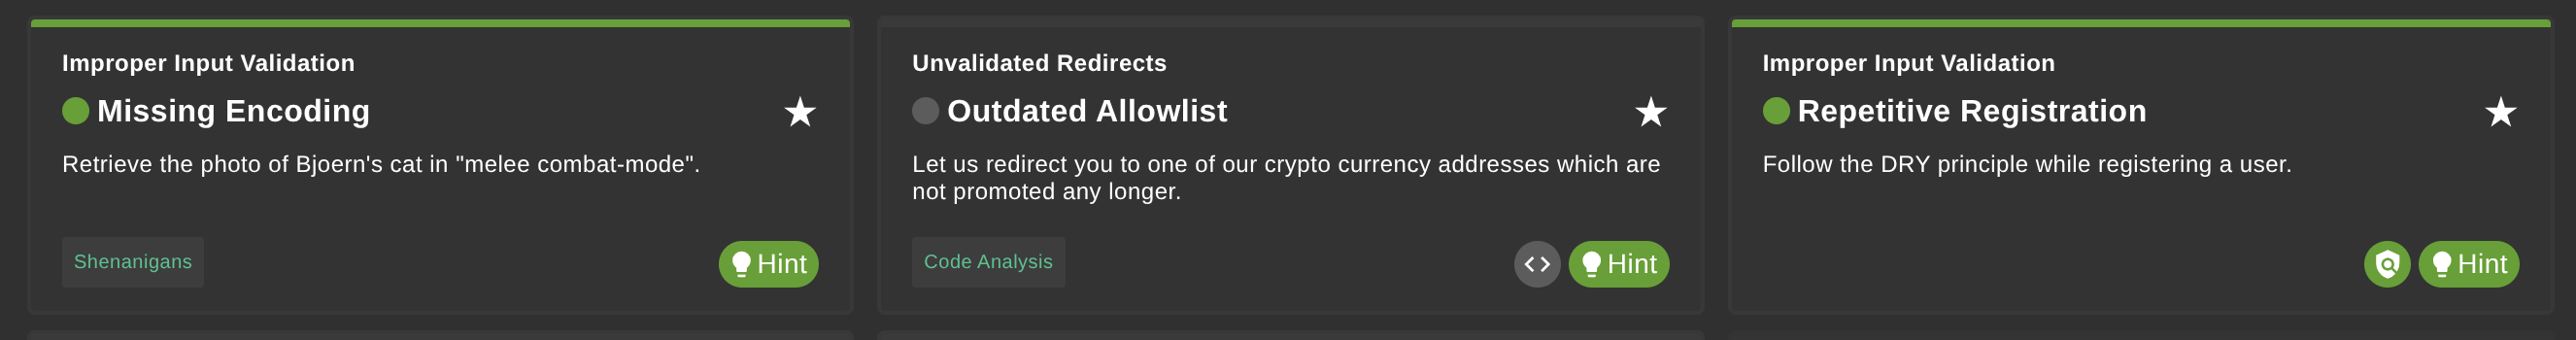
\includegraphics[width=0.5\linewidth]{image.png}
    % \caption{Caption}
\end{figure}
\begin{figure}[H]
    \centering
    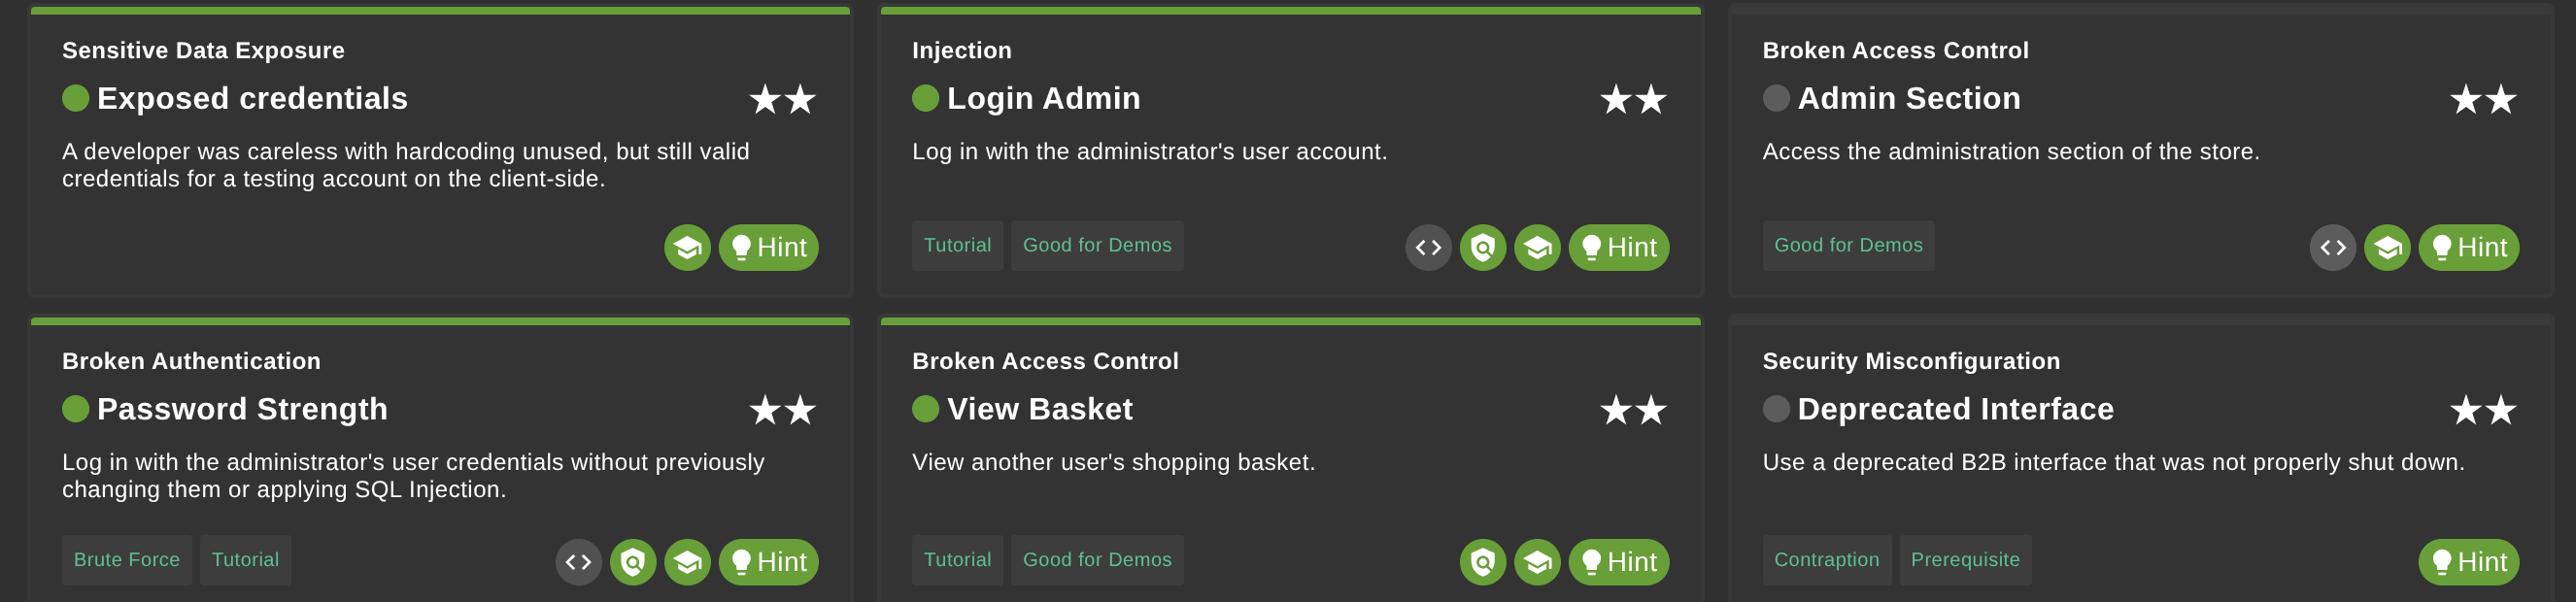
\includegraphics[width=0.5\linewidth]{image copy.png}
    % \caption{Caption}
\end{figure}
\begin{figure}[H]
    \centering
    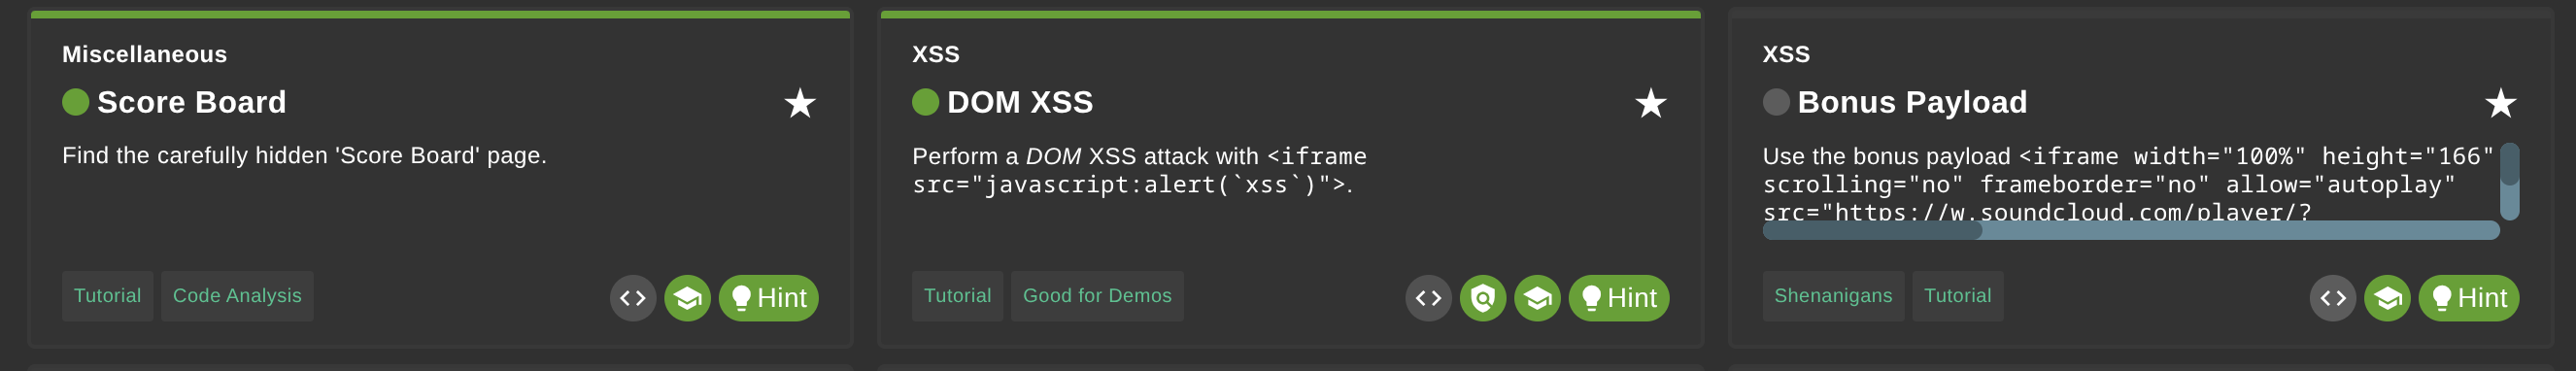
\includegraphics[width=0.5\linewidth]{image copy 2.png}
    % \caption{Caption}
\end{figure}
\subsubsection*{(i) DOM XSS}
Observe that after we search for something, the query keyword we use will be embedded directly in the page. So we can type following text in the searching textbox, the alert function is then successfully triggered.
\begin{minted}[frame=lines,framesep=2mm,baselinestretch=1.2,linenos,breaklines]{html}
<iframe src="javascript:alert(`xss`)">
\end{minted}

The vulnerability introduced is DOM XSS. DOM-based Cross-Site Scripting refers to a type of XSS vulnerability where client-side scripts, usually written in JavaScript, take user-provided input and handle it in an insecure way, resulting in the execution of malicious code within the browser.

To prevent it, we can just validate the input carefully before process it.
\subsubsection*{(v) View Basket}
I open Burp Suite's browser and intercept its traffic, then I observe that when I click \texttt{Your Basket}, there's a GET request contains something like \texttt{GET /rest/basket/1 HTTP/1.1} (if we login admin), then try to change it to 2 or 3 and forward the request, the content of basket is someone else's.

It's a kind of Broken Access Control, the website didn't even validate session or cookie, and encrypt users' information carefully. To solve it, just do the things I just said.
\subsubsection*{(viii) Missing Encoding}
After entering the Photo Wall, we can notice a photo can't be displayed. Inspect the photo's html, we can find its path is not encoded in URL encoding (i.e. percent-encoding), convert the path to correct format using online \href{https://checkserp.com/encode/urlencode/}{tools}, the filename becomes:
\begin{Verbatim}[breaklines]
%e1%93%9a%e1%98%8f%e1%97%a2-%23zatschi-%23whoneedsfourlegs-1572600969477.jpg
\end{Verbatim}

Fill it to original place in html code, we can see the photo is properly displayed!

The problem is classified as Shenanigans (not serious problem), just remind us to encode the filename in URL encoding before put it into the html content.
\subsubsection*{(x) Exposed Credentials}
Open brave browser's Dev tools (Press F12), and then click on \texttt{Sources}, select \texttt{main.js}, search for \texttt{Username} and \texttt{Password}, we can find two lines written \texttt{testingUsername} and \texttt{testingPassword}. 

And then logging in using the password and username we just found. :D
\begin{figure}[H]
    \centering
    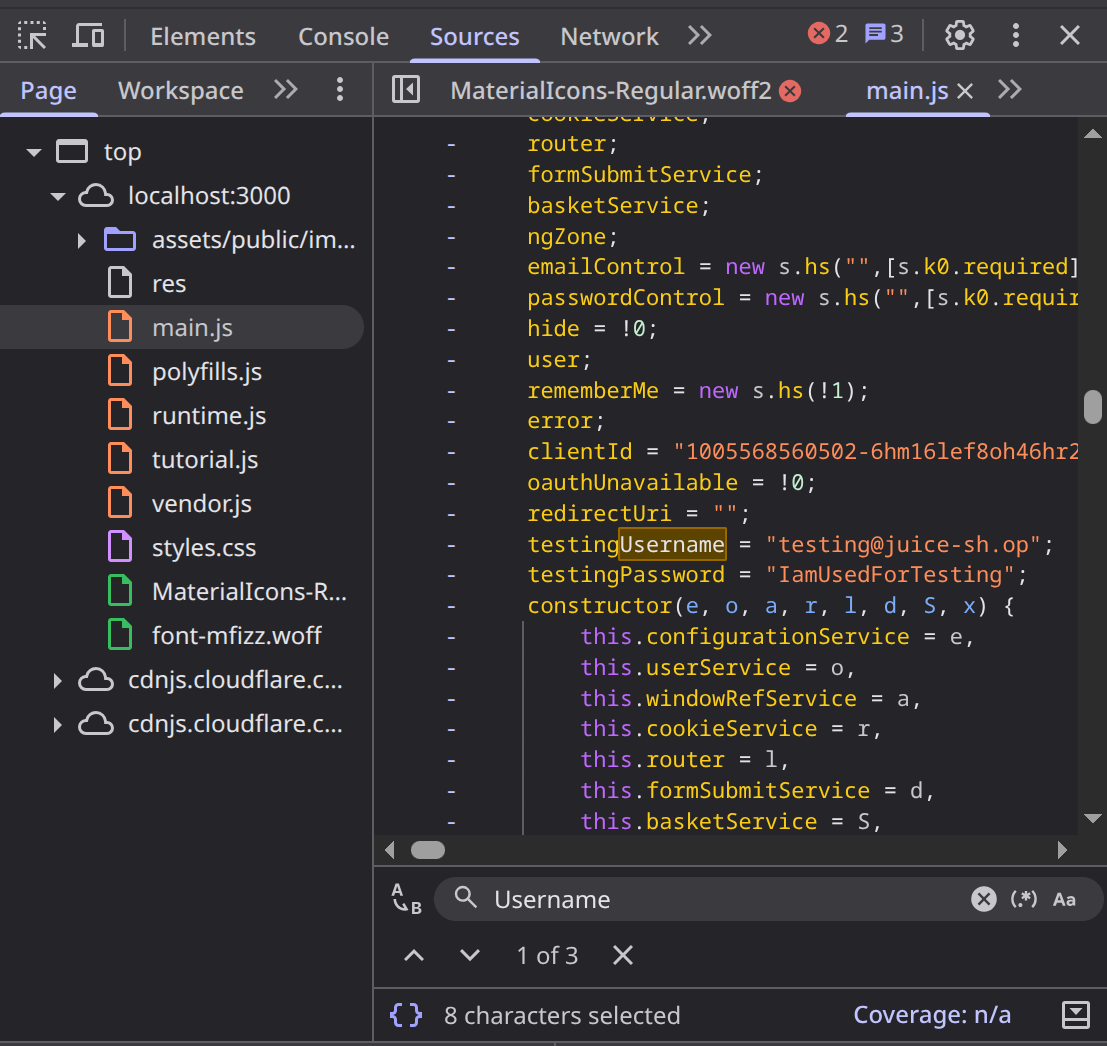
\includegraphics[width=0.5\linewidth]{5.png}
    \caption{Hardcoded username and password in main.js}
\end{figure}

The vulnerability is classified as Sensitive Data Exposure by OWASP juice shop. It's cause by putting sensitive information directly in front-end files instead of storing (and encrypting) it in proper database. To prevent it, just DON't do what I just said.

\subsubsection*{(ix) Repetitive Registration}
Open burpsuite's browser, and then start intercepting it. Register a user normally, in the POST request, edit the content in Repeat Password field to a different one, then forward the request. It's done.

It's a kind of Improper input validation, the website only check the password repetition in the front-end, thus the packet can be intercepted and changed and directly sent to the server. To prevent this, check the content of request (just don't merely check it in front-end) as well.

\subsection*{(b)}
SSRF 是指攻擊者誘使伺服器向內部或外部的目標發出惡意請求,可能用來存取內部資源或發動攻擊。CSRF 則是利用使用者已登入的身份,在未察覺的情況下對其他網站發送請求,執行如轉帳、修改資料等操作。XSS 是指攻擊者將惡意 JavaScript 插入網頁中,當其他使用者瀏覽該頁面時,惡意腳本即在他們的瀏覽器中執行,竊取資料或控制其他操作。

三者的主要差異在於攻擊目標與方式,SSRF 的目標是伺服器,攻擊者利用伺服器對內或對外發起請求。CSRF 的目標是使用者的操作身份,攻擊者偽造合法使用者對網站的操作請求。XSS 的目標是使用者的瀏覽器,攻擊者執行腳本竊取資料或控制其他前端行為。

\newpage
\section*{3. R-SA!破密部}
\subsection*{(a)}
這題的 flag 是:

{\centering\verb|NASA_HW11{blind_signing_is_dangerous}|\par}

假設正整數 $m=m_1*m_2$,而 soyo 的簽名是用 private key $(n,d)$,則根據同餘的乘法性質:
\begin{align*}
m_1^d\equiv a\pmod{n} \\
m_2^d\equiv b\pmod{n} \\
m^d\equiv a*b\pmod{n}
\end{align*}

雖然我們無法取得 \verb|name=soyo| 的 signature,但我們可以先將其轉為大整數,分為兩個因數,再將兩個質因數轉為 byte string 並給 soyo 簽名,最終將兩個餘數相乘 mod n 就等價於 \verb|name=soyo| 的簽章。(我解題的 script 放在 \verb|code/test.py|)

\subsection*{(b)}
這題的 flag 是:

{\centering\verb|NASA_HW11{W0w_y0u_kNow_h@st@d'5_bro4dc@s7_47t@cK}|\par}

根據 anon.py,每次愛音都會利用一組 public key $(n,e)$ 來加密她的 diary,其中 $n$ 是會變的,$e=7$ 是常數。根據 RSA 的一些定義,顯然 $m\le n$ (對每次生成的 $n$ 都是)。By \href{https://cp-algorithms.com/algebra/chinese-remainder-theorem.html}{中國剩餘定理},我們只需要得到 7 個 congruence ($m^7\equiv c_i \pmod{n_i},\ i\in[0,7]$),就能決定唯一的 $m$ ($le$所有 $n$ 的連乘)。我們可以透過類似於 Lagrange interpolation 的方法構造出 $k=m^7$ 的\href{https://cp-algorithms.com/algebra/chinese-remainder-theorem.html}{通解},再取得 $m$ 的值。有了 m 的值,就能將其轉為 byte string 並 decode 了,anyway,最後的結果是正確的 flag,感謝聖愛音。(我解題的 python script 放在 \verb|code/congruence.py|)


\newpage
\section*{4. TESTING in the FUZZ (41 pts)}
\subsection*{(a)}
mutation-based fuzzing is about mutating the existing input values but in lack of understaning the format of the data. generation-based fuzzing is about generating input based on specific or expected format/structure.
\subsection*{(b)}
Greybox fuzzing 是一種結合 black-box 與 white-box 測試特性的 fuzzing。以下是其運作流程 (以 AFL(American Fuzzy Lop)為例):
\begin{enumerate}
    \item 初始輸入:使用者提供一組合法的範例輸入檔(seeds),AFL 從這些檔案開始進行測試。
    \item Instrumentation:AFL 會在目標程式中插入輕量的追蹤程式碼,紀錄執行時的 code coverage。
    \item Mutation:AFL 對現有輸入進行隨機或策略性的變異,如位元翻轉、字元插入、刪除等,產生新測資。
    \item 執行與觀察:AFL 將 mutated input 餵給目標程式,並監控是否產生 crash。若新的輸入觸發了先前未覆蓋的 code coverage,AFL 會將其加入輸入集合,用於後續的變異。
    \item 反覆執行前述的步驟
\end{enumerate}


\newpage
\section*{5. 敗北協定太多了! (28 pts)}
\subsection*{(a)}
攻擊者向 DNS resolver 發送大量的 UDP packet (參數可能是 ANY,讓之後得到的 response 越大越好),將受害者的 IP 放在其中,因此 DNS resolver 將傳送大量的 response 給受害者,可能導致網路、性能遭到癱瘓。

這個攻擊可以透過減少 public DNS resolver 的數量,以及對 source IP 驗證來解決。
\subsection*{(b)}
DNS server 為了加快之後回覆的速度,會存取某 domain 對應到的 IP 作為 cache。Attackers 可以向 DNS server 發出請求,然後當 DNS server 要向 authorative server 請求時,Attackers 可以偽裝成一個合法的 authorative server 向 DNS server 給出扭曲的回應/域名對應到的 IP,也因此 DNS server 之後對於某域名的 cache 都是被污染的。之後受害者去連某域名時,會被 redirect 到駭客提供的 IP。

解決方式可以是透過 DNSSEC 來檢查 DNS 封包的完整性與合法性,或是頻繁更新 DNS cache。
\subsection*{(c)}
SPF 是 \href{https://www.csa.gov.sg/resources/internet-hygiene-portal/information-resources/spf}{Sender Policy Framework} 的縮寫,基本上就是 Domain owner 會在他的 DNS server 發布 SPF record,把 domain name 授權給特定的某幾個 server,接收方的 server 在收到 email 後會去 check 這個信件的 mail server 是不是 Domain 的 SPF record 授權的 server,如果是就接受,如果不是就封鎖或丟到垃圾郵件。
\subsection*{(d)}
DKIM(DomainKeys Identified Mail)是一種電子郵件驗證技術,透過加密簽章確保郵件內容在傳送過程中未被竄改。發信的伺服器會用私鑰對郵件的標頭和部分內容進行簽章,並附加在郵件中。收信伺服器則從發信網域的 DNS 中取得公鑰,用來驗證簽章的真偽。如果簽章驗證成功,就表示郵件確實來自該網域,內容也未被修改。這種機制能有效防止 email spoofing,因為偽造者無法取得合法的私鑰來生成正確的簽章。
\subsection*{(e)}
 在題目所提供的 paper 中有提到,Intra-server attack 是一種利用郵件伺服器內部不同認證模組/協定(如 SPF、DKIM、DMARC)之間解讀不一致的攻擊手法。它們對同一封郵件可能驗證不同的寄件人欄位(如 MAIL FROM 或 HELO)。攻擊者可以設計特殊的郵件格式,例如使用不存在的子網域或特殊字元(如 NUL)來誤導某模組通過驗證。接著,DMARC 可能根據錯誤結果進行比對,使偽造的寄件人地址看似合法。最終結果是郵件通過所有驗證,實際上卻是偽造的寄件者。這種攻擊即使在正確設定 SPF、DKIM、DMARC 的情況下也可能成功,導致 mail spoofing 最終未被成功擋下。
\subsection*{(f)}
TLS 的憑證中會包含 Domain name、Certificate authority、Certificate authority's digital signature、Issuance date、Expiration date、Public key 以及 SSL/TLS version。CA是一個可以信任的第三方機構,負責頒發/簽署 digital certificate 給特定的 domain 或服務。
\subsection*{(g)}
HTTPS downgrade attack 是一種 Man-in-the-middle Attack,攻擊者會攔截使用者與網站之間的連線,並強迫使用者退回使用不安全的 HTTP,從而竊聽或竄改傳輸內容。這種攻擊通常發生在使用者首次連到網站時,若瀏覽器預設使用 HTTP 而非 HTTPS,就有機會被攔截。

作為網站管理員,可以透過一些方式防範這樣的攻擊,例如啟用 HSTS(HTTP Strict Transport Security),讓瀏覽器強制對你的網域使用 HTTPS,並拒絕任何 HTTP 連線。

\newpage
\section*{6. 猫物語(赤)(34 pts)}
\subsection*{(a)}
我得到的 flag 是: \verb|NASA_HW11{pseudorandomness_does_not_guarantee_unpredictability}|. 可以觀察到 fatcat.py 得到 random number 的公式是 $k=(ak+c)\mod{m}$, $k$ 是當前的 state, 其中 $a$ 和 $c$ 是可以透過連續的 3 次 state output 得到的, 假設我們亂猜後得到 3 個正確的 state: $k_1,\ k_2,\ k_3$. 則他們會有以下關係式:
\begin{align*}
    k_2=(ak_1+c)\mod{m} \\
    k_3=(ak_2+c)\mod{m}
\end{align*}

透過一些簡單的數學,我們可以得到 $a=(k_1-k_2)^{-1}(k_2-k_3),\ c=(k_2-ak_1)\mod{m}$ (在這裡 $(k_1-k_2)^{-1}$ 代表其模 $m$ 下的模逆元)。有了 a 和 c 我們就能預測接下來的每個數字,但 trust 要大於等於 100 才會有 flag1,所以我們就用 pwntools 猜 100 多次,再向 server 索取答案。我的 script (放在 \verb|code/guess.py|) 如下所示:
\begin{minted}[frame=lines,framesep=2mm,baselinestretch=1.2,linenos,breaklines]{python}
from pwn import *

server = remote('140.112.91.4', 1234)

server.sendlineafter(b'Your choice: ', b'1')
server.sendlineafter(b'Guess a number: ', b'1')
k1 = int(server.recvuntil(b'.').decode().split(' ')[8].rstrip(','))

server.sendlineafter(b'Your choice: ', b'1')
server.sendlineafter(b'Guess a number: ', b'1')
k2 = int(server.recvuntil(b'.').decode().split(' ')[8].rstrip(','))

server.sendlineafter(b'Your choice: ', b'1')
server.sendlineafter(b'Guess a number: ', b'1')
k3 = int(server.recvuntil(b'.').decode().split(' ')[8].rstrip(','))

m = ... # too long to fit in, but it's given by fatcat.py

a = pow(k1-k2, -1, m) * (k2-k3)
c = (k2-a*k1)%m

cur = k3

for i in range(100):
    server.sendlineafter(b'Your choice: ', b'1')
    cur = (a*cur+c)%m
    server.sendlineafter(b'Guess a number: ', str(cur))

server.sendlineafter(b'Your choice: ', b'2')
flag = server.recvuntil(b'}')
print(flag)
\end{minted}
\subsection*{(b)}
The flag (FLAG2) is \verb|NASA_HW11{07p_k3y_mu57_b3_47_l3457_45_l0n6_45_pl41n73x7}|. Observe that the key is used in a cyclic manner. Since we know the prefix of flag must be \verb|NASA_HW11{|, and its length is equal to the OTP key (it's 10). By xor the string we got in remote server and the prefix, we can obtain the key, thus the original string. But, the flag is not necessarily in first position, so we must enumerate the position of \verb|NASA_HW11{|, and find the one reach the formate requirement and not being meaningless.

My script is put in \verb|code/deOTP.py|, after running it we can find lines written:
\begin{Verbatim}[linenos, breaklines]
b'LinearAlgebraMidterm Name:Fatcat Score:86 Flag:NASA_HW11{07p_k3y_mu57_b3_47_l3457_45_l0n6_45_pl41n73x7}'
\end{Verbatim}
\subsection*{(c)}
The flag (FLAG3) is \verb|NASA_HW11{https://youtu.be/1GxwDuV5JMc}|. Just brute force since $2^{24}$ is not that big, so we can store all the answer and its corresponding key in dictionary. (for simplicity, I don't consider the collisions). My script is shown as below (The file is put in \verb|code/doPoW.py|):
\begin{minted}[frame=lines,framesep=2mm,baselinestretch=1.2,linenos,breaklines]{python}
from pwn import *
import hashlib

mp = dict()
for i in range(2**24):
    mp[hashlib.md5(str(i).encode()).hexdigest()[0:8]] = i

server = remote('140.112.91.4', 1234)
server.sendlineafter(b'Your choice: ', b'4')

for i in range(10):
    prefix = server.recvuntil(b': ').decode().split(' ')[7].strip('"').rstrip('"')
    ans = str(mp[prefix])
    server.sendline(ans)

ans1 = server.recvline()
ans2 = server.recvline()
print(ans1.decode(), ans2.decode())
\end{minted}
\subsection*{(d)}
FLAG4 是 \verb|NASA_HW11{y0u_KN0w_r3F13C710n_4774cK}|,觀察 fatcat.py 可以發現 verify 的時候名字一點都不重要,所以只要讓 sha256 的結果是對的就行,而同時我們要根據 server 給的 nounce 輸入正確的結果,但似乎需要 shared key 欸?其實只要把 nounce 丟進 prover 然後把 server 輸出的 mac 複製下來,再回到 verify 的過程中,輸入 \texttt{richardlaiis||<mac>}, 就可以取得 flag 了,好耶!

\end{document}
% how to display codes?
% \begin{minted}[frame=lines,framesep=2mm,baselinestretch=1.2,linenos,breaklines]{python}
% \end{minted}

% how to display images?
% \begin{figure}[H]
%     \centering
%     \includegraphics[width=0.5\linewidth]{}
%     \caption{Caption}
% \end{figure}
% test